%%%%%%%%%%%%%%%%%%%%%%%%%%%%%%%%%%%%%%%%%%%%%%%%%%%%%%%%%%%%%%%%%%%%%
%
%  This is a sample LaTeX input file for your contribution to 
%  the M&C2019 topical meeting.
%
%  Please use it as a template for your full paper 
%    Accompanying/related file(s) include: 
%       1. Document class/format file: mandc.cls
%       2. Sample Postscript Figure:   figure.pdf
%       3. A PDF file showing the desired appearance: mandc2019_template.pdf
%       4. cites.sty and citesort.sty that might be needed by some users 
%    Direct questions about these files to: palmert@engr.orst.edu
%											mark.dehart@inl.gov
%
%    Notes: 
%      (1) You can use the "dvips" utility to convert .dvi 
%          files to PostScript.  Then, use either Acrobat 
%          Distiller or "ps2pdf" to convert to PDF format. 
%      (2) Different versions of LaTeX have been observed to 
%          shift the page down, causing improper margins.
%          If this occurs, adjust the "topmargin" value in the
%          physor2018.cls file to achieve the proper margins. 
%
%%%%%%%%%%%%%%%%%%%%%%%%%%%%%%%%%%%%%%%%%%%%%%%%%%%%%%%%%%%%%%%%%%%%%


%%%%%%%%%%%%%%%%%%%%%%%%%%%%%%%%%%%%%%%%%%%%%%%%%%%%%%%%%%%%%%%%%%%%%
\documentclass[letterpaper]{mandc2019}
%
%  various packages that you may wish to activate for usage 
\usepackage{tabls}
\usepackage{cites}
\usepackage{epsf}
\usepackage{appendix}
\usepackage{ragged2e}
\usepackage[top=1in, bottom=1.in, left=1.in, right=1.in]{geometry}
\usepackage{enumitem}
\setlist[itemize]{leftmargin=*}
\usepackage{caption}
\captionsetup{width=1.0\textwidth,font={bf,normalsize},skip=0.3cm,within=none,justification=centering}

\usepackage{amsmath}
\usepackage{amsfonts}
\usepackage{amssymb}
\usepackage{amstext}
\usepackage{amsbsy}
\usepackage{bbm}
\usepackage{color}
\usepackage[capitalize]{cleveref}   % smart references - http://ctan.org/pkg/cleveref
\usepackage[bbgreekl]{mathbbol}
\DeclareSymbolFontAlphabet{\mathbbl}{bbold}
\usepackage{xspace}
\usepackage{titlesec}
\usepackage{subcaption}
\usepackage{cite}
\usepackage{multicol}
\newcommand{\angstrom}{\text{\normalfont\AA}}
% Common style and macro defintions for Yak and Mammoth documentation
%=================================================================================================

%%% General Commands
% shortcut for Rattlesnake
\newcommand{\rattlesnake}{Rattlesnake\xspace}
\newcommand{\rsn}{Rattlesnake\xspace}
\newcommand{\MOOSE}{MOOSE\xspace}

%% structural elements
% An explanation for a function
\newcommand{\explain}[1]{\mbox{\hspace{2em} #1}}
% attemtion box
\newcommand{\attention}[1]{\mbox{\hspace{2em} #1}}
% comments at the sde of the paragraph
\newcommand{\sidenotes}[1]{\marginpar{ {\footnotesize #1} }}
% inline comments
\newcommand{\inlinenotes}[1]{{\color{red} {\footnotesize #1} }}
% create empty double page, TODO do we need that?
\newcommand{\clearemptydoublepage}{\newpage{\pagestyle{empty}\cleardoublepage}}
%TODO description here
\newcommand{\apost}{\textit{a posteriori\xspace}}
%TODO description here
\newcommand{\Apost}{\textit{A posteriori}\xspace}
% create a label on text so that it can be later referred with pageref
\newcommand{\hlabel}{\phantomsection\label}

%%% Math
%% Paratnhis etc.
% ()
\newcommand{\parenthesis}[1]{{\left( #1 \right)}}
% []
\newcommand{\bracket}[1]{{\left[ #1 \right]}}
% {}
\newcommand{\bracet}[1]{{\left\{ #1 \right\}}}
% <>
\newcommand{\angled}[1]{{\left\langle #1 \right\rangle}}

%% common math symbols
% imaginary number
\newcommand{\img}{\ensuremath{\hat{\imath}}\xspace}
% gradient symbol
\newcommand{\grad}{\vec{\nabla}}
\newcommand{\del}{\vec{\nabla}}
% adjoint
\newcommand{\adj}[2][{}]{{{#2}^{\dagger #1}}}
% order number
\newcommand{\order}[1]{^\parenthesis{#1}}

%% common math function
% divergence
\renewcommand{\div}{\del\! \cdot \!}
% rotation
\newcommand{\rot}{\del\! \times \!}
% absolute value
\newcommand{\abs}[1]{\left|#1\right|}
% norm
\newcommand{\norm}[2][{}]{\lVert#2\rVert_{#1}}
% e function
\newcommand{\e}[1]{\mathrm{e}^{#1}}
% power of ten
\newcommand{\tento}[1]{\ensuremath{10^{#1}}\xspace}
% E notation
\newcommand{\E}[1]{\ensuremath{\times \tento{#1}}\xspace}
% sign
\DeclareMathOperator{\sign}{sign}

%% fraction
% 1 / 2
\newcommand{\half}[1][1]{\frac{#1}{2}}
% 1 / 3
\newcommand{\third}[1][1]{\frac{#1}{3}}
% 1 / 4
\newcommand{\fourth}[1][1]{\frac{#1}{4}}

% vectors etc
% vector
\newcommand{\vect}[1]{\mathbf{#1}}
\newcommand{\dvect}[1]{\vec{\mathbf{#1}}}
\newcommand{\tvect}[1]{\vec{\vec{\mathbf{#1}}}}
\newcommand{\vectsymbol}[1]{\boldsymbol{#1}}
% matrix
\newcommand{\mat}[1]{\mathbf{#1}}
\newcommand{\vmat}[1]{\vec{\mathbf{#1}}}
\newcommand{\tmat}[1]{\vec{\vec{\mathbf{#1}}}}
% tensor
\newcommand{\tensor}[1]{\vec{\vec{#1}}}
% PDE operator symbol
\newcommand{\op}[1]{\mathbbl{#1}}
% bilinear and linear operator symbol
\newcommand{\kernel}[1]{\mathbbm{#1}}

% derivatives
% first derivatives
% general first derivative, with optional argument for f
\newcommand{\dd}[2][]{\frac{\partial #1}{\partial #2}}
% partial derivative for x, optional argument for f
\newcommand{\ddx}[1][]{\dd[#1]{x}}
% partial derivative for y, optional argument for f
\newcommand{\ddy}[1][]{\dd[#1]{y}}
% partial derivative for z, optional argument for f
\newcommand{\ddz}[1][]{\dd[#1]{z}}
% partial derivative for t, optional argument for f
\newcommand{\ddt}[1][]{\dd[#1]{t}}

% second derivatives, only for a single variable, cross derivatives are too many
% second general derivative, optional argument for f
\newcommand{\ddd}[2][{}]{\frac{\partial^2 #1}{\partial {#2}^2}}
% second partial derivative for x, optional argument for f
\newcommand{\ddxx}[1][]{\ddd[#1]{x}}
% second partial derivative for y, optional argument for f
\newcommand{\ddyy}[1][]{\ddd[#1]{y}}
% second partial derivative for z, optional argument for f
\newcommand{\ddzz}[1][]{\ddd[#1]{z}}
% second partial derivative for t, optional argument for f
\newcommand{\ddtt}[1][]{\ddd[#1]{t}}

% integrals
% integral dx, optional parameter for different variable
\newcommand{\dx}[1][x]{\,d#1}
% integral dy
\newcommand{\dy}{\dx[y]}
% integral dz
\newcommand{\dz}{\dx[z]}
% integral dt
\newcommand{\dt}{\dx[t]}
%integral dmu
\newcommand{\dmu}{\dx[\mu]}
%integral dOmega
\newcommand{\domg}{\dx[\Omega]}

% spherical integrals
% shortcut for sphere notation
\newcommand{\sphere}{\ensuremath{\mathcal{S}}\xspace}
% angular quadrature weight
\newcommand{\aqweight}{\omega}

% integral over full sphere
\newcommand{\intsp}{\int_{4\pi}}
% integral over half sphere
\newcommand{\inthalfsp}{\int_{2\pi}}
% polar integral
\newcommand{\intpolar}{\int_{-1}^{1}}
% negative partial polar integral
\newcommand{\intnpolar}{\int_{-1}^{0}}
% positive partial polar integral
\newcommand{\intppolar}{\int_{0}^{1}}
% positive half sphere with respect to a norm
\newcommand{\intplus}[1]{\int_{\direction\cdot #1 > 0}}
% negative half sphere with respect to a norm
\newcommand{\intminus}[1]{\int_{\direction\cdot #1 < 0}}


% FEM symbols
% spatial domain
\newcommand*{\domain}{\ensuremath{\mathcal{D}}\xspace}
% boundary of a spatical domain
\newcommand*{\boundary}{\ensuremath{{\partial\domain}}\xspace}
% vacuum boundary of a spatical domain
\newcommand*{\vboundary}{\ensuremath{{\boundary}_v}\xspace}
% reflective boundary of a spatical domain
\newcommand*{\rboundary}{\ensuremath{{\boundary}_r}\xspace}
% interface surface
\newcommand*{\interface}{\ensuremath{{\Gamma}}\xspace}
% general and isotropic test function
\newcommand{\testfct}{\ensuremath{\phi^{*}}\xspace}
% angular test function
\newcommand{\atestfct}{\ensuremath{\psi^{*}}\xspace}
% surface normal
\newcommand{\normal}{\ensuremath{\vec{n}}\xspace}
% boundary normal
\newcommand{\bnormal}{\ensuremath{\normal_\mathrm{b}}\xspace}
% surface normal dot direction
\newcommand{\omgdn}{\direction\cdot\normal}
% boundary normal dot direction
\newcommand{\omgdnb}{\direction\cdot\bnormal}

% DFEM commands
% interface jump
\newcommand{\jump}[1]{[\![#1]\!]}
% what is the different?
\newcommand{\jmpa}[1]{[\![\![#1]\!]\!]}
% another jump notation
\newcommand{\jmpb}[1]{\llbracket #1 \rrbracket}
% mean value
\newcommand{\meanval}[1]{\{\!\!\{#1\}\!\!\}}

% common physical symbols
% mass stream
\newcommand{\mdot}{\ensuremath{\dot{m}}\xspace}

% nuclear symbols
% Sn
\newcommand{\sn}[1][N]{\ensuremath{S_#1}\xspace}
% Pn
\newcommand{\pn}[1][N]{\ensuremath{P_#1}\xspace}
% keff
\newcommand{\keff}{\ensuremath{k_{\text{eff}}}\xspace}
% kinf
\newcommand{\kinf}{\ensuremath{k_{\text{inf}}}\xspace}

% transport symbols
% direction omega
\newcommand{\direction}{\ensuremath{\vec{\Omega}}\xspace}
% direction omega
\newcommand{\position}{\ensuremath{\vec{x}}\xspace}
% current
\newcommand{\current}[1][]{\ensuremath{\vec{J}_{#1}}\xspace}
% positive half range current
\newcommand{\ppcurrent}[1][]{\ensuremath{\hat{\jmath}\,^+_{#1}}\xspace}
% negative half range current
\newcommand{\npcurrent}[1][]{\ensuremath{\hat{\jmath}\,^-_{#1}}\xspace}
% drift vector
\newcommand{\drift}[1][]{\ensuremath{\hat{D}_{#1}}\xspace}
% local diffusion coefficient
\newcommand{\DC}[1][]{\ensuremath{\mathrm{D}_{#1}}\xspace}
% nonlocal diffusion tensor
\newcommand{\DCNL}[1][]{\ensuremath{\tensor{\mathrm{D}}_{#1}}\xspace}
% cross section label
\newcommand{\xslabel}[2][]{\ifthenelse{\isempty{#1}}{\mathrm{#2}}{\mathrm{#2},#1}}
% total cross section
\newcommand{\sigt}[1][]{\ensuremath{\sigma_{\xslabel[#1]{t}}}\xspace}
% scattering cross section
\newcommand{\sigs}[1][]{\ensuremath{\sigma_{\xslabel[#1]{s}}}\xspace}
% fission cross section
\newcommand{\sigf}[1][]{\ensuremath{\sigma_{\xslabel[#1]{f}}}\xspace}
% removal cross section
\newcommand{\sigr}[1][]{\ensuremath{\sigma_{\xslabel[#1]{r}}}\xspace}
% absorption cross section
\newcommand{\siga}[1][]{\ensuremath{\sigma_{\xslabel[#1]{a}}}\xspace}
% transport cross section
\newcommand{\sigtr}[1][]{\ensuremath{\sigma_{\xslabel[#1]{tr}}}\xspace}
% scattering moment
\newcommand{\sigl}[2][{}]{\ensuremath{\sigma_{#2#1}}\xspace}
% prompt fission spectrum
\newcommand{\chip}[1][]{\ensuremath{\chi_{\xslabel[#1]{p}}}\xspace}
% delayed fission spectrum
\newcommand{\chid}[1][]{\ensuremath{\chi_{\xslabel[#1]{d}}}\xspace}

% total cross section
\newcommand{\Sigt}[1][]{\ensuremath{\Sigma_{\xslabel[#1]{t}}}\xspace}
% scattering cross section
\newcommand{\Sigs}[1][]{\ensuremath{\Sigma_{\xslabel[#1]{s}}}\xspace}
% fission cross section
\newcommand{\Sigf}[1][]{\ensuremath{\Sigma_{\xslabel[#1]{f}}}\xspace}
% removal cross section
\newcommand{\Sigr}[1][]{\ensuremath{\Sigma_{\xslabel[#1]{r}}}\xspace}
% absorption cross section
\newcommand{\Siga}[1][]{\ensuremath{\Sigma_{\xslabel[#1]{a}}}\xspace}
% transport cross section
\newcommand{\Sigtr}[1][]{\ensuremath{\Sigma_{\xslabel[#1]{tr}}}\xspace}
% scattering moment
\newcommand{\Sigl}[2][{}]{\ensuremath{\Sigma_{#2#1}}\xspace}

% spatial weight function
\newcommand{\weight}[1][]{\ensuremath{w_{#1}}\xspace}

% physical units
% general style for a unit symbol
\newcommand{\unit}[1]{\,\mathrm{#1}}
% distance
% meter maybe \meter better and more clear?
\newcommand{\m}{\unit{m}\xspace}
% centimeter
\newcommand{\cm}{\unit{cm}\xspace}
% milimeter
\newcommand{\mm}{\unit{mm}\xspace}

% time
% second
\newcommand{\s}{\unit{s}\xspace}

% transport units
% scalar flux
\newcommand{\sfluxunit}{\,\ensuremath{\unit{cm}^{-2}\unit{s}^{-1}}\xspace}
% angular flux
\newcommand{\afluxunit}{\,\ensuremath{\unit{cm}^{-2}\unit{s}^{-1}\unit{st}^{-1}}\xspace}
% transport source
\newcommand{\tsrcunit}{\,\ensuremath{\unit{cm}^{-3}\unit{s}^{-1}\unit{st}^{-1}}\xspace}
% diffussion source
\newcommand{\dsrcunit}{\,\ensuremath{\unit{cm}^{-3}\unit{s}^{-1}}\xspace}
% diffusion coefficient
\newcommand{\dcunit}{\,\ensuremath{\unit{cm}}\xspace}


% \newenvironment{myverbatim}%            To change the pseudocode font
% {\par\noindent%
%  \rule[0pt]{\linewidth}{0.2pt}
%  \vspace*{-9pt}
%  \linespread{0.0}\small\verbatim}%
% {\rule[-5pt]{\linewidth}{0.2pt}\endverbatim}
%
% \newenvironment{myverbatim1}%            To change the pseudocode font
% {\par\noindent%
%  \rule[0pt]{\linewidth}{0.2pt}
%  \vspace*{-9pt}
%  \linespread{1.0}\scriptsize\verbatim}%
% {\rule[-5pt]{\linewidth}{0.2pt}\endverbatim}

\newcommand{\source}{Q\xspace}
\newcommand{\n}{d\xspace}
\newcommand{\M}{{N_d}\xspace}

\titleclass{\subsubsubsection}{straight}[\subsection]
\newcounter{subsubsubsection}[subsubsection]
\renewcommand\thesubsubsubsection{\thesubsubsection.\arabic{subsubsubsection}}
\renewcommand\theparagraph{\thesubsubsubsection.\arabic{paragraph}} % optional; useful if paragraphs are to be numbered
\titleformat{\subsubsubsection}
{\normalfont\normalsize\bfseries}{\thesubsubsubsection}{1em}{}
\titlespacing*{\subsubsubsection}
{0pt}{3.25ex plus 1ex minus .2ex}{1.5ex plus .2ex}
\makeatletter
\renewcommand\paragraph{\@startsection{paragraph}{5}{\z@}%
	{3.25ex \@plus1ex \@minus.2ex}%
	{-1em}%
	{\normalfont\normalsize\bfseries}}
\renewcommand\subparagraph{\@startsection{subparagraph}{6}{\parindent}%
	{3.25ex \@plus1ex \@minus .2ex}%
	{-1em}%
	{\normalfont\normalsize\bfseries}}
\def\toclevel@subsubsubsection{4}
\def\toclevel@paragraph{5}
\def\toclevel@paragraph{6}
\def\l@subsubsubsection{\@dottedtocline{4}{7em}{4em}}
\def\l@paragraph{\@dottedtocline{5}{10em}{5em}}
\def\l@subparagraph{\@dottedtocline{6}{14em}{6em}}
\makeatother
\setcounter{secnumdepth}{4}
\setcounter{tocdepth}{4}
\newcommand{\colorsubsubsubsection}[2]{\subsubsubsection{\texorpdfstring{\color{#1}{#2}}{\emph{#2}}}}

\newcommand{\para}[2]{\hyperref[#1]{#2}}


%\usepackage[justification=centering]{caption}

%
% Define title...
%
\title{EFFICIENT SURROGATE FOR LOW ENERGY DAMAGE EFFECTS\\ IN POLYATOMIC MATERIALS}
%
% ...and authors
%
\author{%
  % FIRST AUTHORS 
  %
  \textbf{Sebastian Schunert, Daniel Schwen, Daniel J. Vanwasshenova} \\
  Nuclear Science and Technology Directorate \\
  Idaho National Laboratory \\ Idaho Falls, ID, USA  \\
     \\
     \url{sebastian.schunert@inl.gov}, \url{daniel.schwen@inl.gov} \\ \url{daniel.vanwasshenova@inl.gov} 
}

%
% Insert authors' names and short version of title in lines below
%
\newcommand{\authorHead}      % Author's names here use et al. if more than 3
           {S.Schunert, D. Schwen,  D. J. Vanwasshenova}  
\newcommand{\shortTitle}      % Short title here (Shorten to fit all into a single line)
           {Surrogate for Radiation Damage}  
%%%%%%%%%%%%%%%%%%%%%%%%%%%%%%%%%%%%%%%%%%%%%%%%%%%%%%%%%%%%%%%%%%%%%
%
%   BEGIN DOCUMENT
%
%%%%%%%%%%%%%%%%%%%%%%%%%%%%%%%%%%%%%%%%%%%%%%%%%%%%%%%%%%%%%%%%%%%%%
\begin{document}
\maketitle
\justify 
\allowdisplaybreaks
\begin{abstract}
  We present an efficient surrogate for binary-collision Monte-Carlo (BCMC) calculations in polyatomic materials for low ion energies based on Parkin and Coulter's net displacement function. Most of BCMC's execution time is spent on
  the low energy tail of cascades when recoils' residual travel distance is small
  compared to the desired resolution of the damage calculation. We propose to 
  curtail an ions' random walk if its energy reduces below a threshold $E_t$ and locally deposit an estimate of the expected number of defects it creates; the estimate of the number of defects is obtained from Parkin and Coulter's net displacement functions. We find that results obtained with the BCMC code \textit{MyTRIM} 
  with and without truncation of the random walks compare well for large energy thresholds $E_t > 5$ keV. For $E_t = 5$ keV larger discrepancies are observed because of large differences between the net displacement function and \textit{MyTRIM} for very low energy recoils. Future work will investigate and resolve this discrepancy. The energy threshold should be chosen so that ions' average distance to next nuclear scattering is small compared to the desired resolution. A reduction of execution time of damage cascades by over $90$ \% is observed for an energy threshold of $E_t = 5$ keV and a $1$ MeV Xe-135 primary impinging on UO$_2$.
  The desired application of this surrogate model are coupled FEM-BCMC calculations with varying compositions where net displacement functions are tabulated by composition. For reducing the number of required net displacement functions, derivatives of the net displacement function with respect to number fraction are computed. 
\end{abstract}
\keywords{Radiation damage, Binary-collision Monte-Carlo, Computational Material Science, Net Displacement Function}

%%%%%%%%%%%%%%%%%%%%%%%%%%%%%%%%%%%%%%%%%%%%%%%%%%%%%%%%%%%%%%%%%%%%%%%%%%%%%%%%%%
\section{INTRODUCTION} 
%%%%%%%%%%%%%%%%%%%%%%%%%%%%%%%%%%%%%%%%%%%%%%%%%%%%%%%%%%%%%%%%%%%%%%%%%%%%%%%%%%
The number of displacements caused by primary knock-on atoms (PKA) is of central importance for predicting the evolution of material properties under irradiation. The binary-collision Monte-Carlo (BCMC) method~\cite{SRIM} can be used to simulate representative radiation damage cascades caused by an atom of given type and initial energy. The \textit{SRIM} code~\cite{SRIM} allows computation of spatial distributions of point defects in one-dimensional geometries for polyatomic, amorphous materials. 
The \textit{MyTRIM}~\cite{Schwen2010} code allows BCMC simulations in general, three-dimensional geometries. It is designed to be coupled to mesoscale simulations of nuclear fuel performed with Marmot~\cite{TONKS201220,SCHWEN201736}. The coupling of Marmot and \textit{MyTRIM} is accomplished by the Magpie (\textit{Mesoscale Atomistic Glue Program for Integrated Execution}) code~\cite{Zabriskie2019} that interfaces between the finite element method (FEM) description in Marmot and the discrete representation of defects in \textit{MyTRIM}. 
In Magpie, \textit{MyTRIM} computes point-defect creation rates that are rasterized on a FEM mesh, while Marmot updates material compositions that are used for computing ions' mean free paths.

Binary-collision Monte-Carlo simulations of damage cascades caused by fast ions are computationally expensive. A significant fraction of the execution time is spent on computing the motion of ions at low energies, i.e. late in their life cycle. The damage that these ions cause is spatially clustered and usually confined to a single FEM element. We propose to enhance the efficiency of  BCMC calculations by truncating ion trajectories once their energy reduces below a threshold. The residual point defect production of these ions is estimated using a zero-dimensional radiation damage model.

%In monoatomic materials Kinchin and Pease's work~\cite{Kinchin1955} allows the computation of the number of displacements  
%produced by a collision cascade of hard sphere. 
%Subsequent works refining some assumptions but still limited to monoatomic materials are summarized in~\cite{GaryWas}. 
%The Kinchin-Pease formalism is not sufficient for the purpose of this work because nuclear fuel is never a monoatomic material.

For polyatomic materials, Parkin and Coulter provide integro-differential equations for the net displacement rate~\cite{PC1981} defined as the number of atoms an ion of given type and energy displaces. The net displacement rate is a function of the primary ion's energy only, i.e. it is not a function of space, and the integro-differential equation contains both derivatives and integrals with respect to energy.

In this work, we first introduce the equation for the net displacement rate given by Parkin and Coulter~\cite{PC1981}. 
We present an algorithm for numerically solving the equation for a given material composition. An online computation of the displacement rates is unfeasible and therefore we develop an efficient tabulation algorithm for displacement functions. Instead of storing displacement functions by position, we store them by composition signature and reuse them if the composition of interest is close to any of the compositions in the existing library. The required number of stored damage functions is reduced by using a linear approximation in composition space. The partial derivatives of the displacement function with respect to concentration are computed using linear perturbation theory. 

\section{NET DISPLACEMENT FUNCTIONS} \label{sec:disp_func}
The net displacement rate $g_{ij}(E)$ is defined as the number of atoms of type $j$ displaced and not recaptured by PKA of type $i$ and energy $E$~\cite{PC1981}.
The net displacement function $g_{ij}(E)$ satisfies the equation:
\begin{align}\label{eq:net_pc_1}
  S_{i}(E) \frac{d g_{ij}}{dE}  &= \sum\limits_{k=1}^K \frac{N_k}{N}   
  \left [ A_k(E_k^d, \Lambda_{ik} E) + B_k(0, \Gamma_{ik}(E)) - C_k(0, \Lambda_{ik} E)\right ]\nonumber \\
   A_k(a, b) &= \int\limits_{a}^{b}  \frac{d \sigma_{ik} (E,T)}{dT} g_{kj}(T-E_k^b)  dT \nonumber \\
   B_k(a, b) &= \int\limits_{a}^{b}  \frac{d \sigma_{ik} (E,T)}{dT}  g_{ij}(E-T) dT \nonumber \\
   C_k(a, b) &=  g_{ij}(E) \int\limits_{a}^{b}  \frac{d \sigma_{ik} (E,T)}{dT}   dT,
\end{align}
where $S_i(E) = N \left(\frac{dE}{dx}\right)_i$ is the electronic stopping cross section of species $i$ moving with energy $E$, $N_k$ is the number density of species $k$, $N$ is the total number density of the background material, $\Lambda_{ik} = \frac{4A_i A_j}{(A_i + A_j)^2}$, $A_i$ is the atomic mass of species $i$, $\frac{d \sigma_{ik} (E,T)}{dT}$ is the differential scattering cross section for interaction of species $i$ and $k$ ($i$: projectile, $k$ target), $E_k^d$ is the displacement threshold for species $k$, $E_k^b$ is the binding energy defined as the energy that an atom of type $k$ loses to inelastic processes and lattice vibrations as it is displaced from its lattice position. In addition, $\Gamma_{ik}(E)$ is defined by:
\[
\Gamma_{ik}(E) = \min \left( \Lambda_{ik} E, \max \left( E_k^d, E - E_{ik}^{\text{cap}} \right)  \right),
\]
where $E_{ik}^{\text{cap}}$ is the residual energy threshold of an atom of type $i$ which has displaced an atom of type $k$ to be trapped in the vacant $k$ site.
The initial conditions of Eq.~\ref{eq:net_pc_1} are given by $g_{ij}=\delta_{i,j}~\text{for}~E < \min\limits_i (E_i^d)$.

\subsection{Electronic Stopping and Nuclear Scattering Cross Sections}\label{sec:cross_section}
Material properties enter the net displacement rate equation Eq.~\ref{eq:net_pc_1} in the form of the stopping power $S_i(E)$ and the differential nuclear scattering cross section $\frac{d \sigma_{i,k}(E,T)}{d T}$.
Electronic stopping cross sections are taken from the \textit{MyTRIM} code by dividing the stopping power by the total number density $N$. 
%The stopping powers in \textit{MyTRIM} re-implement the equations also used for \textit{SRIM} and are detailed in~\cite{SRIM}. \textcolor{red}{is that correct?}

The differential scattering cross section is computed using Lindhard's universal representation with the Thomas-Fermi potential~\cite{Lindhard1968}. The universal representation of the scattering cross section is given by:
\begin{equation}\label{eq:universal_scattering_xs}
   \frac{d \sigma_{ij}(E,T)}{dT} = \frac{\pi a^2}{2 T t^{1/2}} f(t^{1/2}),
\end{equation}
where:
\begin{multicols}{2}
\begin{itemize}
  \item $a = 0.8853 a_0 Z^{-1/3}$.
  \item $a_0=0.529177 \angstrom$: Bohr's radius.
  \item $Z =  (Z_i^{2/3} + Z_j^{2/3})^{3/2}$.
  \item $t = \left( \frac{E}{E_L} \right)^2 \frac{T}{T_m}$.
  \item $E_L = \frac{Z_i Z_j e^2}{4 \pi \epsilon_0 a} \frac{A_i + A_j}{A_j}$
  \item $\epsilon_0=8.85 \times10^{-12} \frac{\text{F}}{\text{m}}$: vacuum permittivity.
  \item $T_m = \Lambda_{ij} E$.
\end{itemize}
\end{multicols}
and $f(\xi)$ changes depending on the interaction potential used to evaluate the cross section. For the Thomas-Fermi potential Winterborn, Sigmund, and Sanders~\cite{WSS} find that
\begin{align}\label{eq:WSS}
  f(\xi) &= \gamma ~\xi^{1/3} \left[ 1 + \left( 2 \gamma \xi^{4/3} \right)^{2/3}\right]^{-3/2},
\end{align}
with $\gamma = 1.309$ approximates the exact $f(\xi)$ reasonably well. This work uses Eq.~\ref{eq:WSS} throughout.

Numerical solution of Eq.~\ref{eq:net_pc_1} requires analysis of the asymptotic behavior of $\frac{d \sigma_{ij}(E,T)}{dT}$ as $E, T \rightarrow 0$. To this end, we evaluate Eq.~\ref{eq:universal_scattering_xs} in the limit $t \rightarrow 0$:
\begin{align}
   \lim\limits_{t \rightarrow 0} \frac{f\left(t^{1/2}\right)}{t^{1/2}} &=\gamma t^{-1/3}.
\end{align}
We find that for small $E, T$, Eq.~\ref{eq:universal_scattering_xs} becomes:
\begin{equation}\label{eq:thomas_fermi_lowt}
  \frac{d \sigma_{ij}(E,T)}{dT} =1.309 \frac{\pi a^2}{2}  \left( \frac{A_i}{A_j}\right)^{1/3} \left( \frac{2 Z_i Z_j e^2}{4 \pi \epsilon_0 a} \right)^{2/3} E^{-1/3} T^{-4/3}.
\end{equation}
%To evaluate the scattering cross section in units of $\angstrom^2/\text{eV}$, the following expressions for $E_L$ us useful:
%\begin{equation}
%   E_L = 30.7514664  Z_i  Z_j  Z^{1/3}  \frac{A_i + A_j}{A_j} \text{ eV}.
%\end{equation}

\subsection{Numerical Solution of Net Displacement Equation}\label{sec:cross_section}
In this section the numerical issues with solving Eq.~\ref{eq:net_pc_1} are discussed. 
The main issue is that the interaction cross section becomes unbounded as $T \rightarrow 0$ but we show in this section that the right hand side of Eq.~\ref{eq:net_pc_1} remains bounded. We will start discussing the general numerical approach taken to integrate Eq.~\ref{eq:net_pc_1} first and then highlight the special treatment to ensure numerical stability.

Magpie uses algorithms implemented in the GNU scientific library (GSL)~\cite{GSL} for the solution of the relevant equations.
%The ODE is abstracted into the form
%\begin{equation}\label{eq:general_ode}
%   \frac{d \vec{g}}{dE} = \vec{F} \left( \vec{g},E \right),
%\end{equation}
%where $\vec{g}$ collects the $g_{i,j}$. GSL provides functions to solve Eq.~\ref{eq:general_ode} given the ability to evaluate $\vec{F}$. 
Within this work, the explicit 4th order (classical) Runge-Kutta %(\textit{gsl\_odeiv2\_step\_rk4}) 
is used. Numerical integration of ODEs results in solution on an energy grid denoted by $E_n, n=1,..,N$ where the solution at these points is denoted by $g^{(n)}_{i,j} = g_{i,j}(E_n)$.

Integrals over energy that appear on the right hand side of Eq.~\ref{eq:net_pc_1} are computed as sums of elementary integrals over the range $E_n$ to $E_{n+1}$. The elementary integrals are estimated using GSL's Gauss-Legendre quadrature of order $4$ and the value of $g_{i, j}(E)$ is interpolated linearly using $g^{(n)}_{i,j}$ and $g^{(n+1)}_{i,j}$.

Even though the scattering cross section becomes unbounded for $T \rightarrow 0$, the right hand side of Eq.~\ref{eq:net_pc_1} remains bounded. To demonstrate that, we first rearrange terms:
\begin{align}\label{eq:rearrange}
     B_k(0, \Gamma_{ik}(E)) - C_k(0, \Lambda_{ik} E) = &
     B_k(E_c, \Gamma_{ik}(E)) - C_k(E_c, \Lambda_{ik} E) + \nonumber \\
     &\int\limits_{0}^{E_c} \frac{d \sigma_{ik} (E,T)}{dT} \left( g_{ij}(E-T) - g_{ij}(E) \right) dT,
\end{align}
where $E_c$ is suitably chosen energy cutoff. The apparent singularity is now confined to the last term in Eq.~\ref{eq:rearrange}. 
We will now show that Eq.~\ref{eq:rearrange} is bounded.
Following~\cite{PC1980} we expand the last term into a Taylor series expansion for small $T$:
\begin{equation}\label{eq:taylor}
   g_{ij}(E-T)  - g_{ij}(E) = -T \left . \frac{d g_{ij}}{dE}\right |_{T=0} + \mathcal{O}(T^2).
\end{equation}
Given that the cross sections are of order $T^{-4/3}$, the integrand of the last term is of order $T^{-1/3}$ and thus the integral is bounded.  

It is numerically most favorable to reformulate Eq.~\ref{eq:net_pc_1} by inserting Eq.~\ref{eq:taylor} and solving for $d g_{ij} / dE$:
\begin{equation}\label{eq:damage_energy_function_approx_1}
   \frac{d g_{ij}}{dE} = \frac{\sum\limits_{k=1}^K \frac{N_k}{N}   
  \left [ A_k(E_k^d, \Lambda_{ik} E) + B_k(E_c, \Gamma_{ik}(E)) - C_k(E_c, \Lambda_{ik} E)\right ]}
  {S_i(E) + \sum\limits_{k=1}^K \frac{N_k}{N}  \int\limits_0^{E_c} T \frac{d \sigma_{ik} (E,T)}{dT}   dT}.
\end{equation}

\section{POLYATOMIC PARKIN-COULTER MODEL IN MAGPIE} \label{sec:in_magpie}
The net displacement functions are used as a surrogate for detailed BCMC cascades below a selected energy threshold $E_t$.
Once an ion's energy drops below the energy threshold, the random walk is terminated and an estimate of the expected number of vacancies and interstitials are deposited locally. The local vacancy and interstitial counts $\nu_j$ and $\eta_j$ are incremented by:
\begin{align}\label{eq:below_threshold}
   \nu_j &:= \nu_j + g_{ij}(E) \nonumber \\
   \eta_j &:= \eta_j + g_{ij}(E),
\end{align}
where $i$ is the current ion's type and $E$ its energy.

Displacement functions are tabulated by number fraction. If an ion's random walk is terminated, the local composition is compared with tabulated displacement functions. If a sufficiently good match exists, the existing net displacement function is used in Eq.~\ref{eq:below_threshold}, otherwise a new net displacement function is computed.

The described algorithm is tested on two systems, monoatomic metallic uranium and polyatomic UO$_2$ in a quasi one-dimensional geometry. For both systems, Xe-135 primaries with an energy of $1$ MeV impinge on an infinitely thick target. We tally the linear density of vacancies as a function of penetration depth for different energy thresholds. For UO$_2$, the total vacancy density is obtained by summing the uranium and oxygen vacancy densities. 

The computed vacancy densities plotted versus penetration depth are presented in Figs.~\ref{fig:metal_U} and~\ref{fig:UO2}, respectively. Each plot
contains the \textit{MyTRIM} only calculation indicated by $E_t=0$, \textit{MyTRIM} calculations with random walks truncated at various $E_t > 0$, and finally a case $E_t = 5$ keV$^*$ that stops ions at $5$ keV but does not apply Eq.~\ref{eq:below_threshold}.

\begin{figure}[th]
	\centering
	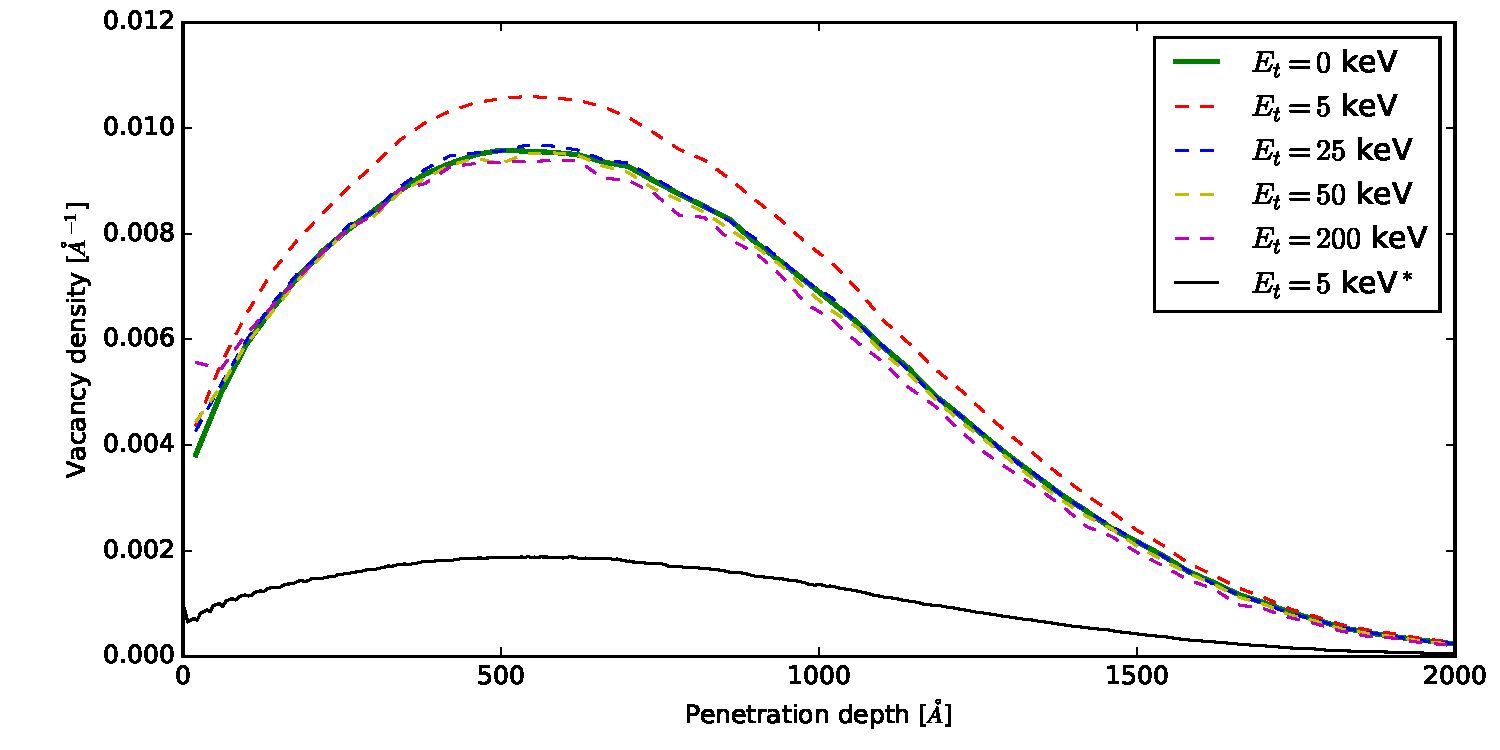
\includegraphics[width=0.9\linewidth]{figures/metal_U.pdf}
	\caption{Linear vacancy density as a function of depth in metallic Uranium created by $1$ MeV Xe-135 ions impinging on the left hand side of the domain. Random walks are terminated if the ion's energy drops below $E_t$ and with the exception of $E_t = 5$ keV$^*$ an estimate of future damage is deposited locally using Eq.~\ref{eq:below_threshold}. \label{fig:metal_U}}
\end{figure}

\begin{figure}[th]
	\centering
	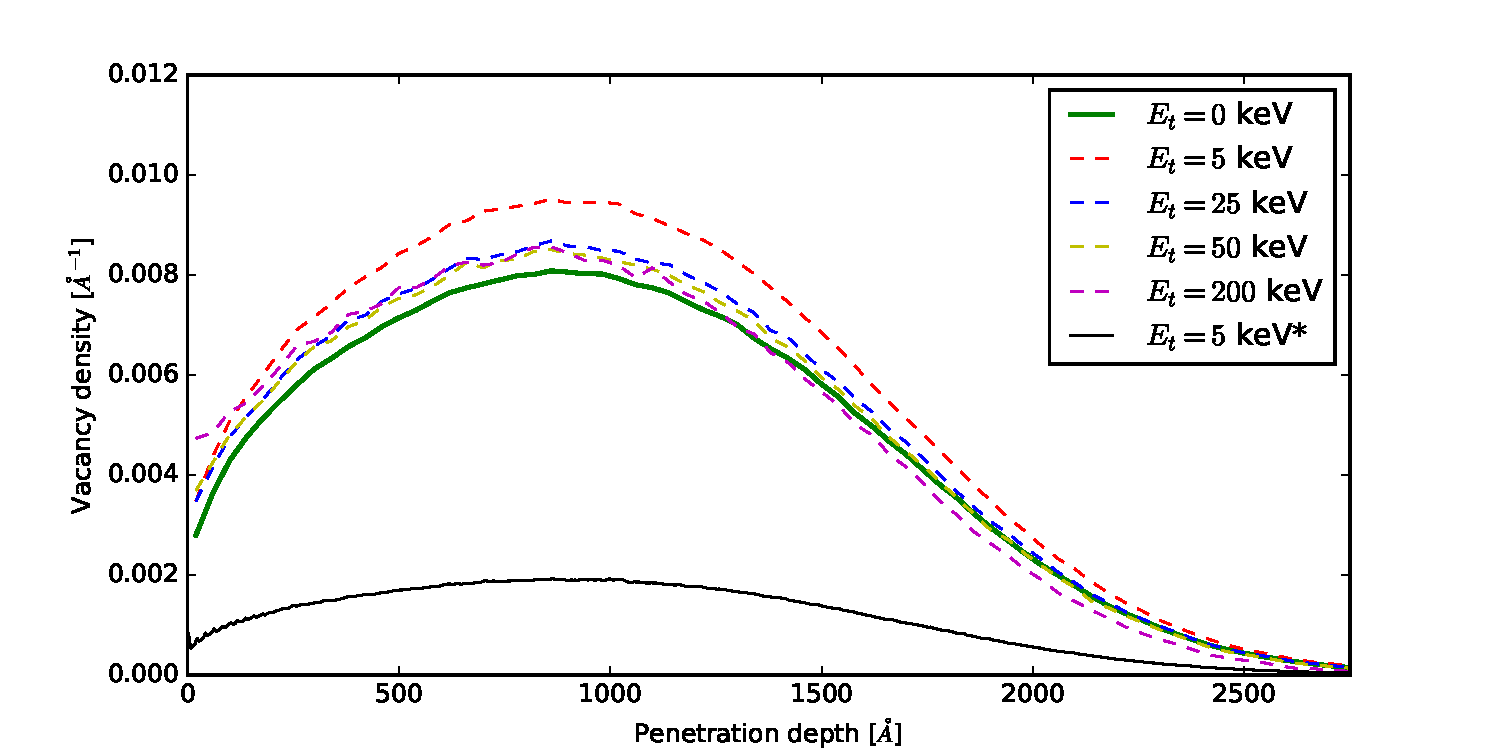
\includegraphics[width=0.9\linewidth]{figures/UO2.pdf}
	\caption{Linear vacancy density as a function of depth in UO$_2$ created by $1$ MeV Xe-135 ions impinging on the left hand side of the domain. The vacancy density is the sum of oxygen and uranium vacancy densities. Random walks are terminated if the ion's energy drops below $E_t$ and with the exception of $E_t = 5$ keV$^*$ an estimate of future damage is deposited locally using Eq.~\ref{eq:below_threshold}.\label{fig:UO2}}
\end{figure}

The vacancy densities with random walks truncated at $E_t$ do not converge to the unmodified \textit{MyTRIM} results as $E_t \rightarrow 0$. This is caused by large differences in the predicted number of defects produced by low energy ions. For $200$ eV uranium projectiles, \textit{MyTRIM} predicts an average of about $0.7$ vacancies per projectile, while Eq.~\ref{eq:net_pc_1} predicts between $1.5$ and $1.6$ vacancies. The large discrepancy of the curves with $E_t = 5$ keV and $E_t=25$ keV is explained as follows: during the damage cascade energy is distributed onto a growing number of particles, so that early in the cascade a few high energy ions exist, and late in the cascade many low energy ions exist. If the energy threshold is chosen at $E_t=5$ keV, we record a large number low energy contributions to $\nu_j$, while we record a small number of large energy contributions at larger $E_t$. For small $E_t$ the differences in \textit{MyTRIM}'s and Eq.~\ref{eq:net_pc_1}'s vacancy yields are amplified by the large number of events leading to a poor prediction of vacancy densities. Currently, this discrepancy is under investigation. It is imperative for the deployment of the truncated cascades that we recover non-truncated \textit{MyTRIM} results as $E_t \rightarrow 0$.

Despite the poor prediction for small $E_t$, the polyatomic Parkin-Coulter formalism gives encouraging results for $E_t\approx 25$ keV. The solid black curves in Figs.~\ref{fig:metal_U} and~\ref{fig:UO2} are the vacancies produced by ions with energies larger than $5$ keV. It is evident that most vacancies are created by ions with $E < 5$ keV and that truncation of their random walks without applying Eq.~\ref{eq:below_threshold} leads to unacceptable errors.

The accuracy of the predicted spatial distribution of vacancies reduces as $E_t$ is increased. Faster ions have larger mean free path. If a fast ion's random walk is curtailed and its future potential for vacancies deposited locally, then the spatial distribution of these vacancies is lost if the mean free path of the ion is comparable or larger than the size of the desired spatial resolution. The spatial resolution is set by the FEM element size that is fixed at $40~\angstrom$ in this work. Uranium ions have a distance between two collisions of the order of $1-5~\angstrom$, while oxygen usually travels more than $10~\angstrom$ between collisions. Therefore, we observe a trend to premature deposition of vacancies in the case of UO$_2$, Fig.~\ref{fig:UO2}. In this case, the total number of predicted vacancies for $E_t=0$ and $E_t=25$ keV is very similar, but when truncating random walks vacancies are created at smaller penetration depths.   

Truncating the random walk has the potential of saving orders of magnitude of execution time without sacrificing accuracy. A cascade of $1$ MeV Xe-135 particles can be executed 12 times faster if $E_t=5$ keV.
This is particularly important for coupled BCMC-FEM calculations where repeated damage cascades for many primary ions have to be completed.

\section{FIRST ORDER PERTURBATION} \label{sec:perturbation}
In this section, we derive an equation for the derivative of the net displacement function with respect to the $l$-th number fraction, i.e. $\theta_{ijl} \equiv \frac{d g_{ij}}{d f_l}$, where $f_l = N_l / N$. The purpose of computing the derivative is to estimate the changes of the net displacement function when the number fractions change. This approach allows to compute fewer net damage functions for spatially distributed radiation damage problems with continuously varying compositions. Future work will use the first order estimate as efficient surrogate for BCMC in coupled FEM-BCMC problems where the composition varies within the domain. 

To first order, changing the number densities $f_l$ to $f_l'$ lead to the following changes in the net displacement rates:
\begin{equation}\label{eq:first_order_net}
   g_{ij} (E,\vec{f}') =  g_{ij} (E,\vec{f}) + \sum\limits_{l=1}^K \theta_{ijl}(E,\vec{f}) (f_l' - f_l) + \mathcal{O}((f_l' - f_l)^2).
\end{equation}
The equations describing the derivative of the net displacement with respect to number fractions is derived using first order perturbation theory. We first introduce a small perturbation $\delta f_l$ that causes a small perturbation in the net displacement function denoted by $\delta g_{ij}^{(l)}$. The perturbation of $f_l$ is chosen to be small enough so that products of two perturbations can be neglected. Substituting:
\begin{align}
   f_k & \leftarrow f_k + \delta f_l ~\delta_{l,k} \nonumber \\
    g_{ij} & \leftarrow g_{ij} + \delta g_{ij}^{(l)} \nonumber \\
    s_i & \leftarrow s_i +\delta s_i^{(l)},
\end{align}
into Eq.~\ref{eq:net_pc_1} leads to an equation for the ratio $\delta g_{ij}^{(l)} / \delta f_l$. The equation for $\theta_{ijl}$ is obtained by passing to the limit $\delta f_l \rightarrow 0$:
\begin{align}\label{eq:net_disp_pert_final}
&   S_i(E)\frac{d \theta_{ijl}}{dE}  
   = \sum\limits_{k=1}^K  f_k \int\limits_{0}^{\Lambda_{ik} E} dT \frac{d \sigma_{ik}}{dT} \Bigg [   \rho_k(T) \theta_{kjl}(T-E_k^b)   
 \nonumber \\
 +& (1 - \rho_k(T) \lambda_{ik}(E-T) )  \theta_{ijl}(E-T)  -\theta_{ijl}(E) \Bigg ]  + Q_{i,j,l}(E)\nonumber \\
 Q_{i,j,l}(E)=&  \int\limits_{0}^{\Lambda_{il} E} dT \frac{d \sigma_{il}}{dT} \Bigg [  \rho_l(T) g_{lj}(T-E_l^b) + (1 - \rho_l(T) \lambda_{il}(E-T) ) g_{ij}(E-T)  - g_{ij}(E) \Bigg ] \nonumber \\
 -& \frac{dS_i(E)}{d f_l}  \frac{d g_{ij}}{dE},
\end{align}
where:
\begin{align}
 \rho_k(T) &= \left\{ \begin{array}{ll}
         0, & ~ T < E_k^d\\
         1, & ~ T \ge E_k^d \end{array} \right.  \nonumber \\
 \lambda_{ik}(E) &=  \left\{ \begin{array}{ll}
         1, & ~ T < E_{ik}^{\text{cap}}\\
         0, & ~ T \ge E_{ik}^{\text{cap}} .\end{array} \right.  
\end{align} 
The initial conditions for the net displacement rates are $g_{ij}(E) = \delta_{ij} \text{ for } E< \min\limits_{i} (E_i^d)$ which are independent of $f_l$. Therefore, the initial condition for $\theta_{ijl}$ is $\theta_{ijl}(E) = 0 \text{ for } E< \min\limits_{i} (E_i^d)$. Equation~\ref{eq:net_disp_pert_final} is identical in form to the original equation for the net displacement function, Eq.~\ref{eq:net_pc_1}, except for the source term $Q_{i,j,l}$. Therefore, solution is straight forward by first obtaining $g_{ij}$ and then using the same algorithm for computing $\theta_{ijl}$ with the only difference that $Q_{ijl}$ is computed from the computed net displacement rate and then added to the right hand side.

We test the correct implementation using $\text{Al}_2\text{O}_3$ as an example. A base case calculation is performed using number fractions of $0.4$ and $0.6$ for Al and O, respectively; then the number fractions are modified to $0.3$ and $0.7$, respectively, corresponding to $\delta f_{\text{Al}} = -0.1$ and $\delta f_{\text{O}} = 0.1$.  The net displacement rates are then (1) re-computed by Eq.~\ref{eq:net_pc_1} using updated number fraction and (2) estimated by Eq.~\ref{eq:first_order_net}. The results are presented in Fig.~\ref{fig:fop_Al2O3}. The markers indicate the direct computation of $g_{ij}$ with modified number fractions, while the dashed-dotted line indicates the estimate using first order perturbation (fop) theory. We observe that estimated and directly computed values agree very well. The limit to which we can use Eq.~\ref{eq:first_order_net} in lieu of computing a new displacement function will be investigated for real systems in future work. It is expected to depend on the desired level of accuracy and the particular material system.

\begin{figure}[th]
	\centering
	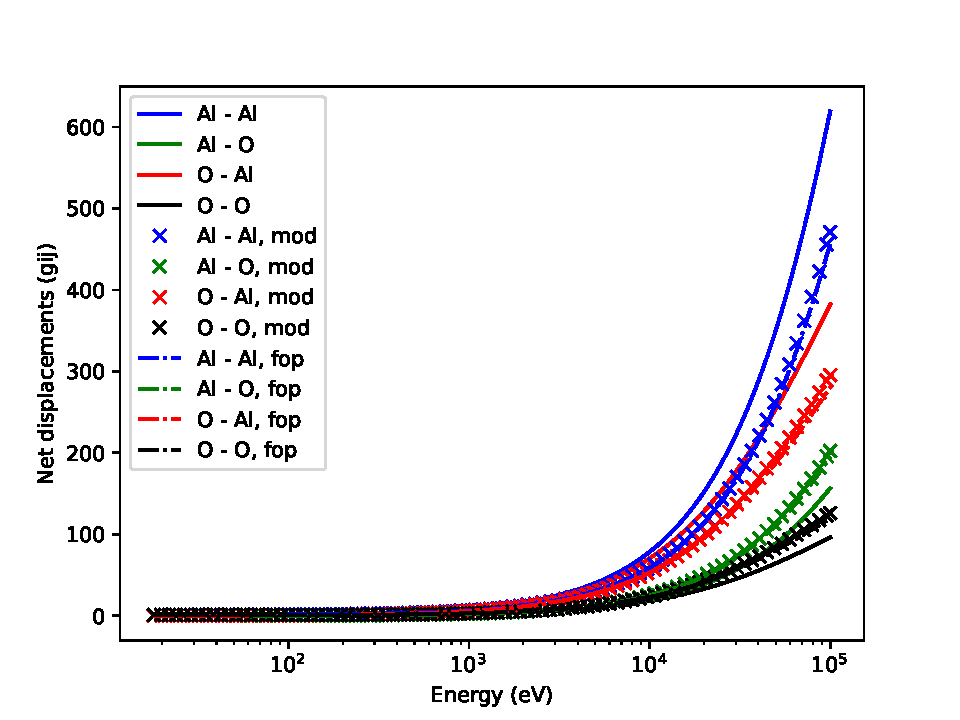
\includegraphics[width=0.7\linewidth]{figures/NRT_first_order_perturbation_theory.pdf}
	\caption{Testing the correctness and precision of estimating the change in net displacement rates of $\text{Al}_2\text{O}_3$ due to changes in number fractions using first order perturbation theory. The solid lines represent $g_{ij}$ for the base number fractions $0.4$/$0.6$, the markers indicate direct computation of the modified system with number fractions $0.3$/$0.7$ (mod), the dashed-dotted lines indicate the estimation using first order perturbation theory (fop).}
	\label{fig:fop_Al2O3}
\end{figure}

\section{CONCLUSIONS} \label{sec:conclusion}
We present an efficient surrogate for low energy damage effects in polyatomic materials. A large portion of the execution time of BCMC calculations is spent on low energy ions that deposit their energy in close proximity of their current location. The Magpie application is designed for solving coupled BCMC-FEM problems, e.g. micro-structure evolution under irradiation. Low energy ions are likely to deposit their energy within a single mesh element so that detailed simulation of ions below a certain energy threshold does not add fidelity to the coupled calculation. Instead of following low energy ions, we propose to terminate ions' random walks and deposit an estimate of the remaining damage locally; the remaining damage is estimated using Parkin and Coulter's net displacement function. Damage functions are stored by composition and reused if an element's composition matches an existing entry's composition sufficiently well. 
We find that results obtained with the BCMC code \textit{MyTRIM} 
  with and without truncation of the random walks compare well for large energy thresholds $E_t > 5$ keV. For $E_t = 5$ keV larger discrepancies are observed because of large differences between the net displacement function and \textit{MyTRIM} for very low energy recoils. Future work will investigate and resolve this discrepancy. The energy threshold should be chosen so that ions' average distance to next nuclear scattering is small compared to the desired resolution. A reduction of execution time of damage cascades by over $90$ \% is observed for an energy threshold of $E_t = 5$ keV for a $1$ MeV Xe-135 primary impinging on UO$_2$.
A linear approximation for computing displacement functions in terms of the number fractions is derived to reduce the number of stored net displacement functions and will be used for coupled FEM-BCMC problems with varying composition.   
 
 \clearpage
\section*{ACKNOWLEDGEMENTS}
This work was supported through the INL Laboratory Directed
Research & Development Program under grant number 16-010.
This work is supported by the U.S. Department of Energy, under DOE
Idaho Operations Office Contract DE-AC07-05ID14517.  Accordingly, the
U.S. Government retains a nonexclusive, royalty-free license to
publish or reproduce the published form of this contribution, or allow
others to do so, for U.S. Government purposes.

\setlength{\baselineskip}{12pt}
\bibliographystyle{mandc}
\bibliography{bibdata}

\end{document}
